% Main-chain revision: AP input -> window -> parameter -> modular Mills.
% Mathematical contracts and proof rows; not kernel-checked Lean.
\documentclass[12pt,reqno]{amsart}
\usepackage{mathtools,adjustbox}
\usepackage{amsfonts}
\usepackage[utf8]{inputenc}
\usepackage{amsmath,amssymb,amsthm}
\usepackage{changepage}
\usepackage{ragged2e}
\usepackage{float}
\usepackage{array}
\usepackage{graphicx}
\usepackage{setspace}
\usepackage{xcolor}
\usepackage{enumitem}
\usepackage[margin=17mm]{geometry}
\setlength{\tabcolsep}{3pt}
\renewcommand{\arraystretch}{1.35}
\renewcommand{\tablename}{$\textsf{Tab}$}
\setlength{\tabcolsep}{3pt}
\renewcommand{\arraystretch}{1.2}
% Tables use simple paragraph columns and one data row per block.
\setcounter{MaxMatrixCols}{20}
\newcommand{\N}{\mathbb N}
\newcommand{\Z}{\mathbb Z}
\newcommand{\Q}{\mathbb Q}
\newcommand{\R}{\mathbb R}
\newcommand{\C}{\mathbb C}
\newcommand{\Np}{\N_{\ge1}}
\newcommand{\fl}[1]{\left\lfloor #1\right\rfloor}

\usepackage{tikz}
\usetikzlibrary{arrows.meta,positioning}
\usepackage{fancyvrb}
\usepackage{fancyhdr}
\usepackage{titlesec,titletoc}
\usepackage[colorlinks=true,linkcolor=blue,citecolor=green,urlcolor=magenta]{hyperref}
\usepackage{aliascnt}
\usepackage[nameinlink]{cleveref}
\usepackage{listings}
\usepackage{booktabs}
\providecommand{\TEXTsymbol}[1]{#1}
% Nonfloating table captions; each simple tabular contains one data row.
\makeatletter
\newcommand{\SplitTableCaption}{\def\@captype{table}\caption}
\makeatother
\restylefloat{figure}
\hypersetup{pageanchor=false}
\makeatletter
\@ifundefined{theorem}{}{\let\theorem\relax}
\@ifundefined{definition}{}{\let\definition\relax}
\@ifundefined{lemma}{}{\let\lemma\relax}
\@ifundefined{corollary}{}{\let\corollary\relax}
\@ifundefined{proposition}{}{\let\proposition\relax}
\@ifundefined{remark}{}{\let\remark\relax}
\@ifundefined{statement}{}{\let\statement\relax}
\makeatother
\DeclareUnicodeCharacter{03B9}{\ensuremath{\iota}}
\DeclareUnicodeCharacter{2200}{\ensuremath{\forall}}
\DeclareUnicodeCharacter{2203}{\ensuremath{\exists }}
\DeclareUnicodeCharacter{2208}{\ensuremath{\in}}
\DeclareUnicodeCharacter{2218}{\ensuremath{\circ}}
\DeclareUnicodeCharacter{2264}{\ensuremath{\leq}}
\DeclareUnicodeCharacter{2265}{\ensuremath{\geq}}
\DeclareUnicodeCharacter{2192}{\ensuremath{\to}}
\DeclareUnicodeCharacter{21A6}{\ensuremath{\mapsto}}
\DeclareUnicodeCharacter{2260}{\ensuremath{\neq}}
\DeclareUnicodeCharacter{00D7}{\ensuremath{\times}}
\DeclareUnicodeCharacter{2115}{\ensuremath{\mathbb{N}}}
\DeclareUnicodeCharacter{211D}{\ensuremath{\mathbb{R}}}
\DeclareUnicodeCharacter{27E8}{\ensuremath{\langle}}
\DeclareUnicodeCharacter{27E9}{\ensuremath{\rangle}}
\providecommand{\period}{\,\allowbreak}
\newcommand{\pagenumside}{C}
\newlength{\pageNumberOffset}
\setlength{\pageNumberOffset}{0pt}
\newcommand{\PagenumSideC}{C}
\newcommand{\applypagehead}[1]{\expandafter\fancyhead\expandafter[\pagenumside]{#1}\ifx\pagenumside\PagenumSideC\else\ifdim\pageNumberOffset=0pt\else\expandafter\fancyheadoffset\expandafter[\pagenumside]{\pageNumberOffset}\fi\fi}
\newcommand{\applypagefoot}[1]{\expandafter\fancyfoot\expandafter[\pagenumside]{#1}\ifx\pagenumside\PagenumSideC\else\ifdim\pageNumberOffset=0pt\else\expandafter\fancyfootoffset\expandafter[\pagenumside]{\pageNumberOffset}\fi\fi}
\pagestyle{fancy}
\fancyhf{}
\applypagehead{\thepage}
\renewcommand{\headrulewidth}{0pt}
\renewcommand{\footrulewidth}{0pt}
\fancypagestyle{plain}{\fancyhf{}\applypagehead{\thepage}\renewcommand{\headrulewidth}{0pt}}
\setlength{\arraycolsep}{1.5pt}
\setlength{\tabcolsep}{1.5pt}
\renewcommand{\arraystretch}{1.0}
\setlength{\arrayrulewidth}{0.4pt}
\setlength{\doublerulesep}{1pt}
\setlength{\extrarowheight}{0pt}
\newcolumntype{C}{>{\centering\arraybackslash\scriptsize}m{40pt}}
\newcolumntype{R}{>{\centering\arraybackslash\scriptsize}m{2.5cm}}
\newcolumntype{L}{>{\centering\arraybackslash\scriptsize}m{10.5cm}}
\fvset{frame=lines,framerule=0.7pt,rulecolor=\color{blue!60!black},framesep=2pt,fontsize=\scriptsize,xleftmargin=4pt,xrightmargin=4pt}
\RecustomVerbatimEnvironment{verbatim}{Verbatim}{}
\DefineVerbatimEnvironment{verbatimbox}{Verbatim}{frame=single,framerule=0.7pt,rulecolor=\color{blue!60!black},framesep=2pt,fontsize=\scriptsize,xleftmargin=4pt,xrightmargin=4pt}
\makeatletter
\def\@setsubjclass{\ifx\@subjclass\@empty\else\@subjclass\fi}
\makeatother
\subjclass{\textbf{2020 Mathematics Subject Classification.}\,Primary 11A41, 11N05.}
\keywords{prime-representing functions, Mills' theorem, arithmetic progressions, short intervals, typed proofs, rational Cauchy codes}
\renewcommand{\abstractname}{\fontsize{9}{11}\selectfont Abstract}
\newcommand{\abstractfont}{\normalfont\fontsize{8}{10}\selectfont}
\newcommand{\abstractheadingsep}{\vspace{0.5em}}
\makeatletter
\renewenvironment{abstract}{\ifx\maketitle\relax\ClassWarning{\@classname}{Abstract should precede\protect\maketitle\space in AMS document classes reported}\fi\global\setbox\abstractbox=\vtop \bgroup\abstractfont{\centering\abstractname\par}\abstractheadingsep\list{}{\labelwidth\z@\leftmargin3pc \rightmargin\leftmargin\listparindent\normalparindent \itemindent\z@\parsep\z@ \@plus\p@\let\fullwidthdisplay\relax}\item\relax}{\endlist\egroup\ifx\@setabstract\relax \@setabstracta \fi}
\makeatother
\setcounter{secnumdepth}{3}
\newcommand{\SecAbove}{1.0ex plus 0.3ex minus 0.1ex}
\newcommand{\SecBelow}{0pt}
\newcommand{\SubsecAbove}{0.8ex plus 0.2ex minus 0.1ex}
\newcommand{\SubsecBelow}{0pt}
\newcommand{\SubsubsecAbove}{0.6ex plus 0.2ex minus 0.1ex}
\newcommand{\SubsubsecBelow}{0pt}
\makeatletter
\titleformat{\section}{\normalfont\fontsize{16}{18}\selectfont\bfseries}{\thesection.}{0.5em}{}
\titleformat{\subsection}{\normalfont\fontsize{14}{16}\selectfont\bfseries}{\thesubsection.}{0.5em}{}
\titleformat{\subsubsection}{\normalfont\fontsize{12}{14}\selectfont\bfseries}{\thesubsubsection.}{0.5em}{}
\titlespacing*{\section}{\z@}{\SecAbove}{\SecBelow}
\titlespacing*{\subsection}{\z@}{\SubsecAbove}{\SubsecBelow}
\titlespacing*{\subsubsection}{\z@}{\SubsubsecAbove}{\SubsubsecBelow}
\makeatother
\newcounter{axctr}\newcounter{posctr}
\newcounter{lemctr}\newcounter{thmctr}\newcounter{asserctr}\newcounter{corctr}
\renewcommand{\theaxctr}{\arabic{axctr}}
\renewcommand{\theposctr}{\arabic{posctr}}
\renewcommand{\thelemctr}{\arabic{lemctr}}
\renewcommand{\thethmctr}{\arabic{thmctr}}
\renewcommand{\theasserctr}{\arabic{asserctr}}
\renewcommand{\thecorctr}{\arabic{corctr}}
\renewcommand{\theHaxctr}{\thesection.\arabic{axctr}}
\renewcommand{\theHposctr}{\thesection.\arabic{posctr}}
\renewcommand{\theHlemctr}{\thesection.\arabic{lemctr}}
\renewcommand{\theHthmctr}{\thesection.\arabic{thmctr}}
\renewcommand{\theHasserctr}{\thesection.\arabic{asserctr}}
\providecommand{\theHasser}{\theequation}
\renewcommand{\theHcorctr}{\thesection.\arabic{corctr}}
\newcommand{\swpax}[2]{\refstepcounter{axctr}\hypertarget{#1}{\mbox{\textbf{Ax\,\theaxctr}}}\label{#2}}
\newcommand{\swppos}[2]{\refstepcounter{posctr}\hypertarget{#1}{\mbox{\textbf{Pos\,\theposctr}}}\label{#2}}
\newcommand{\swplem}[2]{\refstepcounter{lemctr}\hyperlink{#1}{\mbox{\textbf{Lem\,\thelemctr}}}\label{#2}}
\newcommand{\swpthm}[2]{\refstepcounter{thmctr}\hyperlink{#1}{\mbox{\textbf{Thm\,\thethmctr}}}\label{#2}}
\newcommand{\swpcor}[2]{\refstepcounter{corctr}\hypertarget{#1}{\mbox{\textbf{Cor\,\thecorctr}}}\label{#2}}
\newcommand{\tagged}[2]{\hypertarget{#1}{\mbox{\textbf{#2}}}}
\newcommand{\autorefto}[2]{\hyperlink{#1}{#2}}
\newcommand{\mcite}[1]{\text{\cite{#1}}}
\newtheoremstyle{blueplain}{2pt plus 1pt minus 0.5pt}{1pt plus 0.5pt minus 0.3pt}{\itshape}{}{\bfseries\color{blue}}{.}{\newline}{\thmname{#1}\thmnumber{ #2}\thmnote{ {\bfseries\color{blue}(#3)}}}
\theoremstyle{blueplain}
\newtheorem{theorem}{Theorem}[section]
\newtheorem{lemma}{Lemma}[section]
\newtheorem{corollary}{Corollary}[section]
\newtheorem{proposition}{Proposition}[section]
\newtheorem{remark}{Remark}[section]
\newtheorem*{definition}{Definition}
\newtheorem{statement}{Statement}[section]
\definecolor{proofhead}{RGB}{11,83,148}
\definecolor{proofqed}{RGB}{204,0,0}
\renewcommand{\qedsymbol}{\textcolor{proofqed}{\ensuremath{\square}}}
\renewenvironment{proof}[1][Proof]{\par\noindent\textbf{\textcolor{proofhead}{#1.}}\par\nobreak}{\par\nobreak\hfill\qedsymbol}
\newenvironment{swpproof}[1][Proof]{\begin{proof}[#1]}{\end{proof}}
\renewcommand{\theHtheorem}{\thesection.\arabic{theorem}}
\renewcommand{\theHstatement}{\thesection.\arabic{statement}}
\providecommand{\axctrautorefname}{Axiom}
\providecommand{\posctrautorefname}{Postulate}
\providecommand{\lemctrautorefname}{Lemma}
\providecommand{\thmctrautorefname}{Theorem}
\providecommand{\asserctrautorefname}{Proposition}
\providecommand{\corctrautorefname}{Corollary}
\providecommand{\statementautorefname}{Statement}
\crefname{axctr}{axiom}{axioms}
\crefname{posctr}{postulate}{postulates}
\crefname{lemctr}{lemma}{lemmas}
\crefname{thmctr}{theorem}{theorems}
\crefname{asserctr}{proposition}{propositions}
\crefname{corctr}{corollary}{corollaries}
\Crefname{axctr}{Axiom}{Axioms}
\Crefname{posctr}{Postulate}{Postulates}
\Crefname{lemctr}{Lemma}{Lemmas}
\Crefname{thmctr}{Theorem}{Theorems}
\Crefname{asserctr}{Proposition}{Propositions}
\Crefname{corctr}{Corollary}{Corollaries}
\crefname{statement}{statement}{statements}
\Crefname{statement}{Statement}{Statements}
\crefname{section}{section}{sections}
\Crefname{section}{Section}{Sections}
\crefname{equation}{eq}{eqs}
\Crefname{equation}{Eq}{Eqs}
\crefformat{equation}{#2\textcolor{blue}{eq~#1}#3}
\Crefformat{equation}{#2\textcolor{blue}{Eq~#1}#3}
\newcounter{inq}
\renewcommand{\theinq}{\theequation}
\makeatletter
\renewcommand{\p@inq}{\p@equation}
\makeatother
\crefname{inq}{ineq}{inequalities}
\Crefname{inq}{Ineq}{Inequalities}
\crefformat{inq}{#2\textcolor{blue}{inequality~#1}#3}
\Crefformat{inq}{#2\textcolor{blue}{Inequality~#1}#3}
\crefmultiformat{inq}{#2\textcolor{blue}{inequalities~#1}#3}{\textcolor{blue}{ ,\,~#2#1#3}}{\textcolor{blue}{, #2#1#3}}{\textcolor{blue}{ ,\,~#2#1#3}}
\Crefmultiformat{inq}{#2\textcolor{blue}{Inequalities~#1}#3}{\textcolor{blue}{ ,\,~#2#1#3}}{\textcolor{blue}{, #2#1#3}}{\textcolor{blue}{ ,\,~#2#1#3}}
\makeatletter
\newenvironment{ineq}
{\begin{equation}\refstepcounter{inq}}
{\end{equation}}
\makeatother
\newcounter{type}
\renewcommand{\thetype}{\theequation}
\makeatletter
\renewcommand{\p@type}{\p@equation}
\makeatother
\crefname{type}{type}{types}
\Crefname{type}{Type}{Types}
\crefformat{type}{#2\textcolor{blue}{type~#1}#3}
\Crefformat{type}{#2\textcolor{blue}{Type~#1}#3}
\crefmultiformat{type}{#2\textcolor{blue}{types~#1}#3}{\textcolor{blue}{ ,\,~#2#1#3}}{\textcolor{blue}{, #2#1#3}}{\textcolor{blue}{ ,\,~#2#1#3}}
\Crefmultiformat{type}{#2\textcolor{blue}{Types~#1}#3}{\textcolor{blue}{ ,\,~#2#1#3}}{\textcolor{blue}{, #2#1#3}}{\textcolor{blue}{ ,\,~#2#1#3}}
\makeatletter
\newenvironment{type}
{\begin{equation}\refstepcounter{type}}
{\end{equation}}
\makeatother
\newcounter{asser}
\renewcommand{\theasser}{\theequation}
\makeatletter
\renewcommand{\p@asser}{\p@equation}
\makeatother
\crefname{asser}{Assertion}{assertions}
\Crefname{asser}{Assertion}{Assertions}
\crefformat{asser}{#2\textcolor{blue}{assertion~#1}#3}
\Crefformat{asser}{#2\textcolor{blue}{Assertion~#1}#3}
\crefmultiformat{asser}{#2\textcolor{blue}{assertions~#1}#3}{\textcolor{blue}{ ,\,~#2#1#3}}{\textcolor{blue}{, #2#1#3}}{\textcolor{blue}{ ,\,~#2#1#3}}
\Crefmultiformat{asser}{#2\textcolor{blue}{Assertions~#1}#3}{\textcolor{blue}{ ,\,~#2#1#3}}{\textcolor{blue}{, #2#1#3}}{\textcolor{blue}{ ,\,~#2#1#3}}
\makeatletter
\newenvironment{asser}
{\begin{equation}\refstepcounter{asser}}
{\end{equation}}
\makeatother
\newcommand{\thmref}[1]{\hyperref[#1]{Theorem~\ref*{#1}}}
\newcommand{\lemref}[1]{\hyperref[#1]{Lemma~\ref*{#1}}}
\newcommand{\corref}[1]{\hyperref[#1]{Corollary~\ref*{#1}}}
\newcommand{\propref}[1]{\hyperref[#1]{Proposition~\ref*{#1}}}
\makeatletter
\let\orig@maketitle\maketitle
\renewcommand{\maketitle}{\begingroup\let\MakeUppercase\@firstofone\let\uppercase\@firstofone\orig@maketitle\endgroup}
\newlength{\titleToAuthorSkip}
\newlength{\authorToAbstractSkip}
\setlength{\titleToAuthorSkip}{6pt plus 2pt minus 1pt}
\setlength{\authorToAbstractSkip}{10pt plus 3pt minus 2pt}
\renewcommand{\@maketitle}{\normalfont\normalsize\let\@makefnmark\relax\let\@thefnmark\relax\ifx\@empty\@subjclass\else\@footnotetext{\@setsubjclass}\fi\ifx\@empty\@keywords\else\@footnotetext{\@setkeywords}\fi\ifx\@empty\@thanks\else\@footnotetext{\@setthanks}\fi\@settitle\ifx\@empty\@authors\else\vspace{\titleToAuthorSkip}\@setauthors\fi\ifx\@empty\@date\else\vspace{3pt}\@setdate\fi\ifx\@empty\@abstract\else\vspace{\authorToAbstractSkip}\fi\@setabstract}
\makeatother
\makeatletter
\renewcommand{\encodingdefault}{OT1}
\makeatother
\renewcommand{\rmdefault}{cmr}
\renewcommand{\sfdefault}{cmss}
\renewcommand{\ttdefault}{cmtt}
\fontencoding{OT1}\fontfamily{cmr}\selectfont
\renewcommand{\contentsname}{\texorpdfstring{{\color{blue!60!black}\sffamily\Large\selectfont\bfseries Contents}}{Contents}}
\renewcommand{\seriesdefault}{\bfdefault}
\boldmath
\providecommand{\comma}{\allowbreak,\,}
\IfFileExists{tcilatex.tex}{\input{tcilatex}}{}
\makeatletter
\def\dudley@listtighten{  \setlength{\topsep}{0pt}  \setlength{\partopsep}{0pt}  \setlength{\itemsep}{1pt plus 0.5pt minus 0.3pt}  \setlength{\parsep}{0pt}  \setlength{\labelsep}{0.4em}}
\def\dudley@itemlabel{  \ifnum\@listdepth=\@ne \labelitemi
	\else\ifnum\@listdepth=\tw@ \labelitemii
	\else\ifnum\@listdepth=\thr@@ \labelitemiii
	\else \labelitemiv\fi\fi\fi}
\def\dudley@enumlabel{  \ifnum\@listdepth=\@ne \arabic{enumi}.
	\else\ifnum\@listdepth=\tw@ \alph{enumii}.
	\else\ifnum\@listdepth=\thr@@ \roman{enumiii}.
	\else \Alph{enumiv}.\fi\fi\fi}
\def\dudley@enumcounter{  \ifnum\@listdepth=\@ne \usecounter{enumi}  \else\ifnum\@listdepth=\tw@ \usecounter{enumii}  \else\ifnum\@listdepth=\thr@@ \usecounter{enumiii}  \else \usecounter{enumiv}\fi\fi\fi}

\makeatother
\setlength{\parindent}{0pt}
\setlength{\parskip}{0.25em plus 0.05em minus 0.05em}
\makeatletter
\renewenvironment{quotation}
{\list{}{\listparindent\z@
		\itemindent\z@
		\rightmargin\leftmargin
		\parsep\z@}	\item\relax}
{\endlist}
\makeatother
\numberwithin{equation}{section}
\newcolumntype{P}[1]{>{\centering\arraybackslash\scriptsize}m{#1}|}
\lstdefinestyle{python}{
	language=Python,
	basicstyle=\ttfamily\scriptsize,
	keywordstyle=\color{blue},
	commentstyle=\color{gray},
	stringstyle=\color{orange},
	numbers=left,
	numberstyle=\tiny,
	breaklines=true,
	frame=single,
	showstringspaces=false,
	xleftmargin=4pt,
	xrightmargin=4pt
}
\lstdefinestyle{lean}{
	language=ML,
	literate={θ}{{$\theta$}}1 {ε}{{$\varepsilon$}}1 {ℝ}{{$\mathbb R$}}1 {ℕ}{{$\mathbb N$}}1 {ℚ}{{$\mathbb Q$}}1 {·}{{$\cdot$}}1
	{∀}{{$\forall$}}1 {∃}{{$\exists$}}1 {∧}{{$\wedge$}}1
	{→}{{$\to$}}1 {←}{{$\leftarrow$}}1 {≤}{{$\le$}}1
	{⌊}{{$\lfloor$}}1 {⌋}{{$\rfloor$}}1 {₊}{{$_+$}}1
	{⟨}{{$\langle$}}1 {⟩}{{$\rangle$}}1,
	basicstyle=\ttfamily\scriptsize,
	keywordstyle=\color{blue},
	commentstyle=\color{gray},
	stringstyle=\color{orange},
	numbers=left,
	numberstyle=\tiny,
	breaklines=true,
	frame=single,
	showstringspaces=false,
	xleftmargin=4pt,
	xrightmargin=4pt
}
\setcounter{tocdepth}{1}
\contentsmargin{1em}
\titlecontents{part}[0pt]{\addvspace{14pt}\large\bfseries}{\makebox[2.0em][l]{\thecontentslabel.}}{}{\titlerule*[0.6pc]{.}\contentspage}[\addvspace{4pt}]
\titlecontents{section}[2.0em]{\addvspace{10pt}\small\bfseries}{\makebox[2.0em][l]{\thecontentslabel.}}{\hspace*{-2.0em}}{\titlerule*[0.6pc]{.}\contentspage}[\addvspace{2pt}]
\titlecontents{subsection}[4.5em]{\addvspace{4pt}\footnotesize}{\makebox[2.5em][l]{\thecontentslabel.}}{\hspace*{-2.5em}}{\titlerule*[0.6pc]{.}\contentspage}[\addvspace{1pt}]
\setlist[itemize]{topsep=0pt,partopsep=0pt,itemsep=1pt plus 0.5pt minus 0.3pt,parsep=0pt,leftmargin=1.5em,labelsep=0.4em,label=\textbullet}
\setlist[enumerate]{topsep=0pt,partopsep=0pt,itemsep=1pt plus 0.5pt minus 0.3pt,parsep=0pt,leftmargin=1.8em,labelsep=0.4em}


% Predicate display expressions are written directly in hyperlinks.
\newcommand{\defitem}[2]{\hypertarget{def:#1}{#2}}
\newcommand{\proofitem}[2]{\hypertarget{proof:#1}{#2}}
\DeclareRobustCommand{\proofref}[2]{\hyperlink{proof:#1}{\ensuremath{#2}}}
% Suppress hyperlinks, but retain displayed names, in PDF bookmark strings.
\pdfstringdefDisableCommands{%
  \def\proofref#1#2{#2}%
  \def\hyperlink#1#2{#2}}


% Exact row navigation: range links lead to the first row of the cited range.
\newcommand{\DeclareProofBlock}[2]{%
  \expandafter\def\csname ProofBlockName@#1\endcsname{#2}}
\newcommand{\stepitem}[3]{\hypertarget{proofstep:#1:#2}{#3}}
\DeclareRobustCommand{\stepref}[2]{%
  \hyperlink{proofstep:#1:#2}{\ensuremath{\csname ProofBlockName@#1\endcsname(#2)}}}
\DeclareRobustCommand{\steprangeref}[3]{%
  \hyperlink{proofstep:#1:#2}{\ensuremath{\csname ProofBlockName@#1\endcsname(#2\text{--}#3)}}}


% One measured maximum for every formula; never exceed the local column.
\newlength{\FormulaMaxWidth}
\setlength{\FormulaMaxWidth}{0.90\textwidth}
\newlength{\FormulaFitWidth}
\DeclareRobustCommand{\FormulaFit}[2][\displaystyle]{%
  \begingroup
  \setlength{\FormulaFitWidth}{\dimexpr\linewidth-4pt\relax}%
  \ifdim\hsize<\linewidth
    \setlength{\FormulaFitWidth}{\dimexpr\hsize-4pt\relax}%
  \fi
  \ifdim\FormulaFitWidth>\FormulaMaxWidth
    \setlength{\FormulaFitWidth}{\FormulaMaxWidth}%
  \fi
  \mathord{\hbox{%
    \adjustbox{max width=\FormulaFitWidth}{%
      $\mathsurround=0pt #1 #2$}%
  }}%
  \endgroup
}

\begin{document}
\title{\huge Modular Mills' Theorem\\[10pt]
 {\large A Typed Mathematical Presentation}}

\author{ 
	\bfseries{\large \hspace{1.2in} Brahimi Mahdi Tahar\newline\text{ \
		} \newline\text{ \  } \hspace{0.5in}\text{ \  } University of Mohamed
		Boudiaf of M'sila, Algeria\newline\text{ \  }
		\newline\href{mailto:mahditahar.brahimi@univ-msila.dz}{mahditahar.brahimi@univ-msila.dz}}
}


\begin{abstract}
\centering
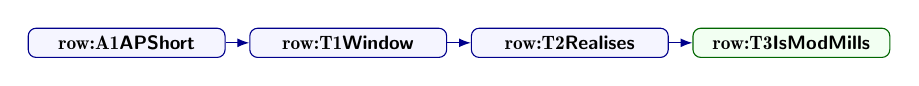
\begin{tikzpicture}[node distance=3mm,
 dep/.style={draw=blue!55!black,fill=blue!4,rounded corners=1mm,
 text width=23mm,align=center,font=\scriptsize,inner sep=1mm},
 done/.style={dep,draw=green!40!black,fill=green!5},
 flow/.style={-{Latex[length=1.5mm]},blue!55!black}]
\node[dep] (a) {\hyperlink{row:A1}{\textsf{APShort}}};
\node[dep,right=of a] (w) {\hyperlink{row:T1}{\textsf{Window}}};
\node[dep,right=of w] (p) {\hyperlink{row:T2}{\textsf{Realises}}};
\node[done,right=of p] (m) {\hyperlink{row:T3}{\textsf{IsModMills}}};
\draw[flow] (a)--(w);
\draw[flow] (w)--(p);
\draw[flow] (p)--(m);
\end{tikzpicture}
\par\medskip\noindent\textit{This is typed mathematical exposition, not kernel-checked Lean. The finite algorithms take a supplied window threshold; the analytic argument supplies no certified numerical value here.}
\end{abstract}
\maketitle
\thispagestyle{empty}
%\newpage
%\thispagestyle{empty}
\bigskip\tableofcontents\bigskip
%\newpage

\setstretch{1.2}\pagestyle{plain}\pagenumbering{arabic}
\hypersetup{pageanchor=true}
\section{Definitions}\label{sec:defs}
\begingroup
\scriptsize
\setlength{\parskip}{0pt}
\noindent
\begin{tabular}{|@{}p{0.19251\linewidth}|p{0.16845\linewidth}|p{0.53904\linewidth}|}\hline
{\hypertarget{def:Scalars}{\(\textsf{Scalars}\)}} & {\(\textsf{Type}\)} & {\(\displaystyle \N,\Z,\Q,\R:\textsf{Type},\quad\N\hookrightarrow\Z\hookrightarrow\Q\hookrightarrow\R,\)
\par
\(\displaystyle \iota_{\N\Z}:\N\to\Z,\quad\iota_{\N\Q}:\N\to\Q,\)
\par
\(\displaystyle \iota_{\N\R}:\N\to\R,\quad\iota_{\Q\R}:\Q\to\R,\)
\par
\(\displaystyle \widehat n:=\iota_{\N\R}(n)\quad(n:\N),\)
\par
\(\displaystyle \lfloor\cdot\rfloor:\R\to\Z,\quad\lfloor\cdot\rfloor_{\N},\lceil\cdot\rceil_{\N}:\R_{\ge0}\to\N.\)}\\
\hline
\end{tabular}%
\par\setlength{\parskip}{0pt}\nointerlineskip
\noindent
\begin{tabular}{|@{}p{0.19251\linewidth}|p{0.16845\linewidth}|p{0.53904\linewidth}|}\hline
{\hypertarget{def:Nat.Prime}{\(\textsf{Nat.Prime}\)}} & {\(\N\to\textsf{Prop}\)} & {\(\displaystyle \forall p:\N,\quad \hyperlink{def:Nat.Prime}{\ensuremath{\textsf{Nat.Prime}}}(p)\Longleftrightarrow\)
\par
\(\displaystyle 2\le p\ \wedge\ \forall d:\N,\ d\mid p\Rightarrow(d=1\vee d=p).\)}\\
\hline
\end{tabular}%
\par\setlength{\parskip}{0pt}\nointerlineskip
\noindent
\begin{tabular}{|@{}p{0.19251\linewidth}|p{0.16845\linewidth}|p{0.53904\linewidth}|}\hline
{\hypertarget{def:Nat.Coprime}{\(\textsf{Nat.Coprime}\)}} & {\(\N\to\N\to\textsf{Prop}\)} & {\(\displaystyle \forall a,m:\N,\quad \hyperlink{def:Nat.Coprime}{\ensuremath{\textsf{Nat.Coprime}}}(a,m)\Longleftrightarrow\gcd(a,m)=1.\)}\\
\hline
\end{tabular}%
\par\setlength{\parskip}{0pt}\nointerlineskip
\noindent
\begin{tabular}{|@{}p{0.19251\linewidth}|p{0.16845\linewidth}|p{0.53904\linewidth}|}\hline
{\hypertarget{def:Nat.ModEq}{\(\textsf{Nat.ModEq}\)}} & {\(\N\to\N\to\N\to\textsf{Prop}\)} & {\(\displaystyle \forall m,p,a:\N,\quad \hyperlink{def:Nat.ModEq}{\ensuremath{\textsf{Nat.ModEq}}}(m,p,a)\Longleftrightarrow\)
\par
\(\displaystyle p\bmod m=a\bmod m.\)}\\
\hline
\end{tabular}%
\par\setlength{\parskip}{0pt}\nointerlineskip
\noindent
\begin{tabular}{|@{}p{0.19251\linewidth}|p{0.16845\linewidth}|p{0.53904\linewidth}|}\hline
{\hypertarget{def:PrimeClass}{\(\textsf{PrimeClass}\)}} & {\(\N\to\N\to\N\to\textsf{Prop}\)} & {\(\displaystyle \forall m,a,p:\N,\quad \hyperlink{def:PrimeClass}{\ensuremath{\textsf{PrimeClass}}}_{m,a}(p)\Longleftrightarrow\)
\par
\(\displaystyle \hyperlink{def:Nat.Prime}{\ensuremath{\textsf{Nat.Prime}}}(p)\wedge \hyperlink{def:Nat.ModEq}{\ensuremath{\textsf{Nat.ModEq}}}(m,p,a).\)}\\
\hline
\end{tabular}%
\par\setlength{\parskip}{0pt}\nointerlineskip
\noindent
\begin{tabular}{|@{}p{0.19251\linewidth}|p{0.16845\linewidth}|p{0.53904\linewidth}|}\hline
{\hypertarget{def:APRange}{\(\textsf{APRange}\)}} & {\(\N\to\R\to\R\to\textsf{Prop}\)} & {\(\displaystyle \forall m:\N\ \forall\alpha,X_0:\R,\quad \hyperlink{def:APRange}{\ensuremath{\textsf{APRange}}}_{m,\alpha}(X_0)\Longleftrightarrow\)
\par
\(\displaystyle \forall x:\R_{\ge2}\ \forall h:\R\ \forall b:\N,\)
\par
\(\displaystyle \bigl[X_0\le x\wedge x^\alpha\le h\le x\wedge b<m\)
\par
\(\displaystyle \wedge \hyperlink{def:Nat.Coprime}{\ensuremath{\textsf{Nat.Coprime}}}(b,m)\bigr]\Rightarrow\)
\par
\(\displaystyle \exists r:\N,\ \hyperlink{def:PrimeClass}{\ensuremath{\textsf{PrimeClass}}}_{m,b}(r)\wedge x-h<r\le x.\)}\\
\hline
\end{tabular}%
\par\setlength{\parskip}{0pt}\nointerlineskip
\noindent
\begin{tabular}{|@{}p{0.19251\linewidth}|p{0.16845\linewidth}|p{0.53904\linewidth}|}\hline
{\hypertarget{def:APShort}{\(\textsf{APShort}\)}} & {\(\N\to\R\to\textsf{Prop}\)} & {\(\displaystyle \forall m:\N\ \forall\alpha:\R,\quad \hyperlink{def:APShort}{\ensuremath{\textsf{APShort}}}_m(\alpha)\Longleftrightarrow\)
\par
\(\displaystyle 2\le m\wedge0<\alpha<1\wedge\)
\par
\(\displaystyle \exists X_0:\R,\ 2\le X_0\wedge \hyperlink{def:APRange}{\ensuremath{\textsf{APRange}}}_{m,\alpha}(X_0).\)}\\
\hline
\end{tabular}%
\par\setlength{\parskip}{0pt}\nointerlineskip
\noindent
\begin{tabular}{|@{}p{0.19251\linewidth}|p{0.16845\linewidth}|p{0.53904\linewidth}|}\hline
{\hypertarget{def:Window}{\(\textsf{Window}\)}} & {\(\N\to\N\to\N\to\textsf{Prop}\)} & {\(\displaystyle \forall c,m,N:\N,\quad \hyperlink{def:Window}{\ensuremath{\textsf{Window}}}_c(m,N)\Longleftrightarrow\)
\par
\(\displaystyle 2\le c\wedge2\le m\wedge2\le N\wedge\)
\par
\(\displaystyle \forall p,a:\N,\ N\le p\Rightarrow \hyperlink{def:Nat.Coprime}{\ensuremath{\textsf{Nat.Coprime}}}(a,m)\Rightarrow\)
\par
\(\displaystyle \exists r:\N,\ \hyperlink{def:PrimeClass}{\ensuremath{\textsf{PrimeClass}}}_{m,a}(r)\wedge p^c<r\le(p+1)^c-2.\)}\\
\hline
\end{tabular}%
\par\setlength{\parskip}{0pt}\nointerlineskip
\noindent
\begin{tabular}{|@{}p{0.19251\linewidth}|p{0.16845\linewidth}|p{0.53904\linewidth}|}\hline
{\hypertarget{def:IsModMills}{\(\textsf{IsModMills}\)}} & {\(\N\to\N\to\N\to\R\to\textsf{Prop}\)} & {\(\displaystyle \forall c,m,a:\N\ \forall A:\R,\quad \hyperlink{def:IsModMills}{\ensuremath{\textsf{IsModMills}}}_{c,m,a}(A)\Longleftrightarrow\)
\par
\(\displaystyle 1<A\ \wedge\ \forall i:\N\ \exists p:\N,\)
\par
\(\displaystyle \hyperlink{def:PrimeClass}{\ensuremath{\textsf{PrimeClass}}}_{m,a}(p)\wedge\lfloor A^{c^{i+1}}\rfloor=\iota_{\N\Z}(p).\)}\\
\hline
\end{tabular}%
\par\setlength{\parskip}{0pt}\nointerlineskip
\noindent
\begin{tabular}{|@{}p{0.19251\linewidth}|p{0.16845\linewidth}|p{0.53904\linewidth}|}\hline
{\hypertarget{def:IRoot}{\(\textsf{IRoot}\)}} & {\(\N\to\Np\to\N\)} & {\(\displaystyle \forall M,k:\N\ \forall e:\Np,\)
\par
\(\displaystyle k=\hyperlink{def:IRoot}{\ensuremath{\textsf{IRoot}}}(M,e)\Longleftrightarrow k^e\le M<(k+1)^e.\)}\\
\hline
\end{tabular}%
\par\setlength{\parskip}{0pt}\nointerlineskip
\noindent
\begin{tabular}{|@{}p{0.19251\linewidth}|p{0.16845\linewidth}|p{0.53904\linewidth}|}\hline
{\hypertarget{def:FastCauchy}{\(\textsf{FastCauchy}\)}} & {\((\N\to\Q)\to\textsf{Prop}\)} & {\(\displaystyle \forall z:\N\to\Q,\quad \hyperlink{def:FastCauchy}{\ensuremath{\textsf{FastCauchy}}}(z)\Longleftrightarrow\)
\par
\(\displaystyle \forall s,t:\N,\ s\le t\Rightarrow|z_s-z_t|\le2^{-s}.\)}\\
\hline
\end{tabular}%
\par\setlength{\parskip}{0pt}\nointerlineskip
\noindent
\begin{tabular}{|@{}p{0.19251\linewidth}|p{0.16845\linewidth}|p{0.53904\linewidth}|}\hline
{\hypertarget{def:Realises}{\(\textsf{Realises}\)}} & {\((\N\to\Q)\to\R\to\textsf{Prop}\)} & {\(\displaystyle \forall z:\N\to\Q\ \forall A:\R,\quad \hyperlink{def:Realises}{\ensuremath{\textsf{Realises}}}(z,A)\Longleftrightarrow\)
\par
\(\displaystyle \forall\varepsilon:\R,\ 0<\varepsilon\Rightarrow\exists S:\N,\)
\par
\(\displaystyle \forall s:\N,\ S\le s\Rightarrow|\iota_{\Q\R}(z_s)-A|<\varepsilon.\)}\\
\hline
\end{tabular}%
\par\setlength{\parskip}{0pt}\nointerlineskip
\noindent
\begin{tabular}{|@{}p{0.19251\linewidth}|p{0.16845\linewidth}|p{0.53904\linewidth}|}\hline
{\hypertarget{def:head}{\(\textsf{head}\)}} & {\(\forall L:\textsf{List}(\N),\ L\ne[]\to\N\)} & {\(\displaystyle \forall x:\N\ \forall L:\textsf{List}(\N)\ \forall h:(x::L)\ne[],\)
\par
\(\displaystyle \hyperlink{def:head}{\ensuremath{\textsf{head}}}(x::L,h)=x,\)
\par
\(\displaystyle \forall L:\textsf{List}(\N)\ \forall h:L\ne[],\)
\par
\(\displaystyle \textsf{List.Mem}(\hyperlink{def:head}{\ensuremath{\textsf{head}}}(L,h),L).\)}\\
\hline
\end{tabular}%
\par\setlength{\parskip}{0pt}\nointerlineskip
\noindent
\begin{tabular}{|@{}p{0.19251\linewidth}|p{0.16845\linewidth}|p{0.53904\linewidth}|}\hline
{\hypertarget{def:Above}{\(\textsf{Above}\)}} & {\(\N\to\textsf{Type}\)} & {\(\displaystyle \forall N:\N,\quad \hyperlink{def:Above}{\ensuremath{\textsf{Above}}}(N):=\textsf{Subtype}(\lambda p:\N,\ N\le p),\)
\par
\(\displaystyle t:\hyperlink{def:Above}{\ensuremath{\textsf{Above}}}(N)\Rightarrow\)
\par
\(\displaystyle t.\textsf{val}:\N,\quad t.\textsf{property}:N\le t.\textsf{val}.\)}\\
\hline
\end{tabular}
\par\setlength{\parskip}{0pt}\nointerlineskip
\noindent
\begin{tabular}{|@{}p{0.19251\linewidth}|p{0.16845\linewidth}|p{0.53904\linewidth}|}\hline
{\hypertarget{def:Totient}{\(\varphi\)}} & {\(\N_{\ge2}\to\Np\)} & {\(\displaystyle \forall m:\N_{\ge2},\quad\varphi(m):=\textsf{List.length}\)
\par
\(\displaystyle \bigl(\textsf{List.filter}(\lambda b:\N,\ \textsf{decide}(\hyperlink{def:Nat.Coprime}{\ensuremath{\textsf{Nat.Coprime}}}(b,m)))\)
\par
\(\displaystyle (\textsf{List.range}(m))\bigr),\qquad1\le\varphi(m).\)}\\
\hline
\end{tabular}
\par\setlength{\parskip}{0pt}\nointerlineskip
\noindent
\begin{tabular}{|@{}p{0.19251\linewidth}|p{0.16845\linewidth}|p{0.53904\linewidth}|}\hline
{\hypertarget{def:Theta}{\(\Theta\)}} & {\(\N\to\N\to\R_{\ge2}\to\R\to\R\)} & {\(\displaystyle \forall m,b:\N\ \forall x:\R_{\ge2}\ \forall h:\R,\)
\par
\(\displaystyle \Theta_{m,b}(x,h):=\sum_{p=2}^{\lfloor x\rfloor_{\N}}\)
\par
\(\displaystyle \textsf{ite}(\hyperlink{def:PrimeClass}{\ensuremath{\textsf{PrimeClass}}}_{m,b}(p)\wedge x-h<p,\ \log p,\ 0).\)}\\
\hline
\end{tabular}
\par\setlength{\parskip}{0pt}\nointerlineskip
\noindent
\begin{tabular}{|@{}p{0.19251\linewidth}|p{0.16845\linewidth}|p{0.53904\linewidth}|}\hline
{\hypertarget{def:LogScale}{\(\mathcal L\)}} & {\(\R_{\ge\mathrm e^{\mathrm e}}\to\R_{>0}\)} & {\(\displaystyle \forall x:\R_{\ge\mathrm e^{\mathrm e}},\quad\mathcal L(x):=\frac{(\log x)^{1/3}}{(\log\log x)^{1/3}}.\)}\\
\hline
\end{tabular}
\par\setlength{\parskip}{0pt}\nointerlineskip
\noindent
\begin{tabular}{|@{}p{0.19251\linewidth}|p{0.16845\linewidth}|p{0.53904\linewidth}|}\hline
{\hypertarget{def:APEstimate}{\(\textsf{APEstimate}\)}} & {\(\N_{\ge2}\to\R\to\R\to\R\to\textsf{Prop}\)} & {\(\displaystyle \forall m:\N_{\ge2}\ \forall C,\kappa,T:\R,\)
\par
\(\displaystyle \hyperlink{def:APEstimate}{\ensuremath{\textsf{APEstimate}}}_m(C,\kappa,T)\Longleftrightarrow\)
\par
\(\displaystyle 0<C\wedge0<\kappa\wedge\mathrm e^{\mathrm e}\le T\ \wedge\)
\par
\(\displaystyle \forall x:\R_{\ge\mathrm e^{\mathrm e}}\ \forall h:\R_{>0}\ \forall b:\N,\)
\par
\(\displaystyle \bigl[T\le x\wedge m\le\log x\wedge x^{29/48}\log x\le h\le x\)
\par
\(\displaystyle \wedge b<m\wedge \hyperlink{def:Nat.Coprime}{\ensuremath{\textsf{Nat.Coprime}}}(b,m)\bigr]\Rightarrow\)
\par
\(\displaystyle \left|\frac{\hyperlink{def:Totient}{\varphi(m)}\hyperlink{def:Theta}{\Theta_{m,b}(x,h)}}h-1\right|\)
\par
\(\displaystyle \le C\exp\bigl(-\kappa \hyperlink{def:LogScale}{\mathcal L(x)}\bigr).\)}\\
\hline
\end{tabular}
\par
\endgroup
\section{Analytic Input and Real Completeness}\label{sec:axioms}
\begingroup
\scriptsize
\setlength{\parskip}{0pt}
\noindent
\begin{tabular}{|@{}p{0.10658\linewidth}|p{0.03553\linewidth}|p{0.52105\linewidth}|p{0.23684\linewidth}|}\hline
{\hypertarget{row:S1}{\(\textsf{S}\)}} & {1} & {\(\displaystyle \varepsilon_0:\R:=1/48,\quad0<\varepsilon_0<5/12,\)
\par
\(\displaystyle 7/12+\varepsilon_0=29/48,\)
\par
\(\displaystyle \forall m:\N,\quad2\le m\Rightarrow\exists C,\kappa,T:\R,\)
\par
\(\displaystyle \hyperlink{def:APEstimate}{\ensuremath{\textsf{APEstimate}}}_m(C,\kappa,T).\)} & {\cite{ThornerZaman2024} \hyperlink{abbr-source:ThornerZaman2024}{\ensuremath{\textsf{Thm}_{1.1},\textsf{Rem}_{1.2},\textsf{Sec}_{1.2}}} \hyperlink{def:APEstimate}{\ensuremath{\textsf{APEstimate}}}}\\
\hline
\end{tabular}%
\par\setlength{\parskip}{0pt}\nointerlineskip
\noindent
\begin{tabular}{|@{}p{0.10658\linewidth}|p{0.03553\linewidth}|p{0.52105\linewidth}|p{0.23684\linewidth}|}\hline
{\hypertarget{row:C1}{\(\textsf{C}\)}} & {1} & {\(\displaystyle \forall z:\N\to\Q,\quad \hyperlink{def:FastCauchy}{\ensuremath{\textsf{FastCauchy}}}(z)\Rightarrow\)
\par
\(\displaystyle \exists!A:\R,\ \hyperlink{def:Realises}{\ensuremath{\textsf{Realises}}}(z,A).\)} & {\hyperlink{def:Scalars}{\ensuremath{\textsf{Scalars}}} \hyperlink{def:FastCauchy}{\ensuremath{\textsf{FastCauchy}}} \hyperlink{def:Realises}{\ensuremath{\textsf{Realises}}}}\\
\hline
\end{tabular}%
\par
\endgroup
\section{Lemmas and Theorems}\label{sec:theorems}
\begin{proposition}[Fixed-modulus AP consequence]\label{prop:ap-input}
\begingroup\scriptsize\setlength{\parskip}{0pt}\noindent
\begin{tabular}{|@{}p{0.10658\linewidth}|p{0.03553\linewidth}|p{0.52105\linewidth}|p{0.23684\linewidth}|}\hline
{\hypertarget{row:A1}{\(\textsf{A}\)}} & {1} & {\(\displaystyle \forall m:\N,\quad2\le m\Rightarrow \hyperlink{def:APShort}{\ensuremath{\textsf{APShort}}}_m(5/8).\)} & {\hyperlink{row:E5}{\ensuremath{\textsf{E}_{5}}}}\\
\hline
\end{tabular}
\par\endgroup
\end{proposition}

\begin{lemma}[AP input to prime windows]\label{lem:ap-window}
\begingroup
\scriptsize
\setlength{\parskip}{0pt}
\noindent
\begin{tabular}{|@{}p{0.10658\linewidth}|p{0.03553\linewidth}|p{0.52105\linewidth}|p{0.23684\linewidth}|}\hline
{\hypertarget{row:T1}{\(\textsf{T}\)}} & {1} & {\(\displaystyle \forall c,m:\N,\quad3\le c\Rightarrow2\le m\Rightarrow\)
\par
\(\displaystyle \hyperlink{def:APShort}{\ensuremath{\textsf{APShort}}}_m(5/8)\Rightarrow\exists N:\N,\ \hyperlink{def:Window}{\ensuremath{\textsf{Window}}}_c(m,N).\)} & {\hyperlink{row:W10}{\ensuremath{\textsf{W}_{10}}}}\\
\hline
\end{tabular}%
\par
\endgroup
\end{lemma}
\begin{lemma}[Prime windows to parameter construction]\label{lem:typed-window-limit}
\begingroup
\scriptsize
\setlength{\parskip}{0pt}
\noindent
\begin{tabular}{|@{}p{0.10658\linewidth}|p{0.03553\linewidth}|p{0.52105\linewidth}|p{0.23684\linewidth}|}\hline
{\hypertarget{row:T2}{\(\textsf{T}\)}} & {2} & {\(\displaystyle \forall c,m,a,N:\N,\quad3\le c\Rightarrow2\le m\Rightarrow\)
\par
\(\displaystyle \hyperlink{def:Nat.Coprime}{\ensuremath{\textsf{Nat.Coprime}}}(a,m)\Rightarrow \hyperlink{def:Window}{\ensuremath{\textsf{Window}}}_c(m,N)\Rightarrow\)
\par
\(\displaystyle \exists A:\R,\ \hyperlink{def:IsModMills}{\ensuremath{\textsf{IsModMills}}}_{c,m,a}(A).\)} & {\hyperlink{row:P19}{\ensuremath{\textsf{P}_{19}}}}\\
\hline
\end{tabular}%
\par
\endgroup
\end{lemma}
\begin{theorem}[Modular Mills theorem]\label{thm:mod-global}
\begingroup
\scriptsize
\setlength{\parskip}{0pt}
\noindent
\begin{tabular}{|@{}p{0.10658\linewidth}|p{0.03553\linewidth}|p{0.52105\linewidth}|p{0.23684\linewidth}|}\hline
{\hypertarget{row:T3}{\(\textsf{T}\)}} & {3} & {\(\displaystyle \forall c,m,a:\N,\quad3\le c\Rightarrow2\le m\Rightarrow\)
\par
\(\displaystyle \hyperlink{def:Nat.Coprime}{\ensuremath{\textsf{Nat.Coprime}}}(a,m)\Rightarrow\exists A:\R,\ \hyperlink{def:IsModMills}{\ensuremath{\textsf{IsModMills}}}_{c,m,a}(A).\)} & {\hyperlink{row:M1}{\ensuremath{\textsf{M}_{1}}}}\\
\hline
\end{tabular}%
\par
\endgroup
\end{theorem}
\section{Proofs}\label{sec:proofs}
\subsection{Derivation of the analytic corollary}\label{sec:analytic-corollary}
\begingroup\scriptsize\setlength{\parskip}{0pt}\noindent
\begin{tabular}{|@{}p{0.10658\linewidth}|p{0.03553\linewidth}|p{0.52105\linewidth}|p{0.23684\linewidth}|}\hline
{\hypertarget{row:E1}{\(\textsf{E}\)}} & {1} & {\(\displaystyle m:\N,\quad h_m:2\le m,\quad C,\kappa,T:\R,\)
\par
\(\displaystyle \eta_{\mathrm{TZ}}:\hyperlink{def:APEstimate}{\ensuremath{\textsf{APEstimate}}}_m(C,\kappa,T)\quad[\exists\textsf{E}],\)
\par
\(\displaystyle 0<C,\quad0<\kappa,\quad\mathrm e^{\mathrm e}\le T.\)} & {\hyperlink{row:S1}{\ensuremath{\textsf{S}_{1}}} \hyperlink{def:APEstimate}{\ensuremath{\textsf{APEstimate}}}}\\
\hline
\end{tabular}
\par\setlength{\parskip}{0pt}\nointerlineskip
\noindent
\begin{tabular}{|@{}p{0.10658\linewidth}|p{0.03553\linewidth}|p{0.52105\linewidth}|p{0.23684\linewidth}|}\hline
{\hypertarget{row:E2}{\(\textsf{E}\)}} & {2} & {\(\displaystyle \forall x:\R,\quad\mathrm e^{4608}\le x\Rightarrow\)
\par
\(\displaystyle t:=\log x\ge4608,\quad\exp(t/48)\ge t^2/4608\ge t,\)
\par
\(\displaystyle \log x\le x^{1/48},\qquad x^{29/48}\log x\le x^{5/8}.\)} & {\hyperlink{row:E1}{\ensuremath{\textsf{E}_{1}}}}\\
\hline
\end{tabular}
\par\setlength{\parskip}{0pt}\nointerlineskip
\noindent
\begin{tabular}{|@{}p{0.10658\linewidth}|p{0.03553\linewidth}|p{0.52105\linewidth}|p{0.23684\linewidth}|}\hline
{\hypertarget{row:E3}{\(\textsf{E}\)}} & {3} & {\(\displaystyle B:=\max\bigl(1,\log(2C)/\kappa\bigr),\)
\par
\(\displaystyle X_{\mathrm{err}}:=\exp\bigl(\max(16,B^6)\bigr),\)
\par
\(\displaystyle \forall x:\R,\quad X_{\mathrm{err}}\le x\Rightarrow\)
\par
\(\displaystyle u:=\log x\ge16,\quad v:=\log u\ge0,\)
\par
\(\displaystyle \exp(v/2)\ge1+v/2+v^2/8>v,\)
\par
\(\displaystyle 0<\log\log x\le\sqrt{\log x},\)
\par
\(\displaystyle \hyperlink{def:LogScale}{\mathcal L(x)}\ge(\log x)^{1/6}\ge B,\)
\par
\(\displaystyle C\exp(-\kappa\mathcal L(x))\le C\exp(-\kappa B)\le1/2.\)} & {\hyperlink{row:E1}{\ensuremath{\textsf{E}_{1}}} \hyperlink{def:LogScale}{\ensuremath{\textsf{LogScale}}}}\\
\hline
\end{tabular}
\par\setlength{\parskip}{0pt}\nointerlineskip
\noindent
\begin{tabular}{|@{}p{0.10658\linewidth}|p{0.03553\linewidth}|p{0.52105\linewidth}|p{0.23684\linewidth}|}\hline
{\hypertarget{row:E4}{\(\textsf{E}\)}} & {4} & {\(\displaystyle X_0:=\max\bigl(T,\mathrm e^m,\mathrm e^{4608},X_{\mathrm{err}}\bigr)\ge2,\)
\par
\(\displaystyle \forall x,h:\R\ \forall b:\N,\)
\par
\(\displaystyle \bigl[X_0\le x\wedge x^{5/8}\le h\le x\wedge b<m\)
\par
\(\displaystyle \wedge \hyperlink{def:Nat.Coprime}{\ensuremath{\textsf{Nat.Coprime}}}(b,m)\bigr]\Rightarrow\)
\par
\(\displaystyle 0<h,\quad m\le\log x,\quad x^{29/48}\log x\le h,\)
\par
\(\displaystyle \left|\frac{\varphi(m)\Theta_{m,b}(x,h)}h-1\right|\le1/2,\)
\par
\(\displaystyle \Theta_{m,b}(x,h)\ge\frac h{2\varphi(m)}>0.\)} & {\hyperlink{row:S1}{\ensuremath{\textsf{S}_{1}}} \hyperlink{row:E1}{\ensuremath{\textsf{E}_{1}}} \hyperlink{row:E2}{\ensuremath{\textsf{E}_{2}}} \hyperlink{row:E3}{\ensuremath{\textsf{E}_{3}}} \hyperlink{def:Totient}{\ensuremath{\textsf{Totient}}} \hyperlink{def:Theta}{\ensuremath{\textsf{Theta}}}}\\
\hline
\end{tabular}
\par\setlength{\parskip}{0pt}\nointerlineskip
\noindent
\begin{tabular}{|@{}p{0.10658\linewidth}|p{0.03553\linewidth}|p{0.52105\linewidth}|p{0.23684\linewidth}|}\hline
{\hypertarget{row:E5}{\(\textsf{E}\)}} & {5} & {\(\displaystyle \forall x:\R_{\ge2}\ \forall h:\R\ \forall b:\N,\)
\par
\(\displaystyle 0<\Theta_{m,b}(x,h)\Rightarrow\exists r:\N,\)
\par
\(\displaystyle \hyperlink{def:PrimeClass}{\ensuremath{\textsf{PrimeClass}}}_{m,b}(r)\wedge x-h<r\le x,\)
\par
\(\displaystyle \rho:\hyperlink{def:APRange}{\ensuremath{\textsf{APRange}}}_{m,5/8}(X_0),\)
\par
\(\displaystyle \hyperlink{def:APShort}{\ensuremath{\textsf{APShort}}}_m(5/8)\quad[\exists\textsf{I},\wedge\textsf{I},\forall\textsf{I}].\)} & {\hyperlink{row:E1}{\ensuremath{\textsf{E}_{1}}} \hyperlink{row:E4}{\ensuremath{\textsf{E}_{4}}} \hyperlink{def:Theta}{\ensuremath{\textsf{Theta}}} \hyperlink{def:APRange}{\ensuremath{\textsf{APRange}}} \hyperlink{def:APShort}{\ensuremath{\textsf{APShort}}}}\\
\hline
\end{tabular}
\par\endgroup

\subsection{AP input to prime windows}\label{sec:ap-window-proof}
\begingroup
\scriptsize
\setlength{\parskip}{0pt}
\noindent
\begin{tabular}{|@{}p{0.10658\linewidth}|p{0.03553\linewidth}|p{0.52105\linewidth}|p{0.23684\linewidth}|}\hline
{\hypertarget{row:W1}{\(\textsf{W}\)}} & {1} & {\(\displaystyle c,m:\N,\quad\gamma:3\le c,\quad\mu:2\le m,\)
\par
\(\displaystyle \eta_{\mathrm{AP}}:\hyperlink{def:APShort}{\ensuremath{\textsf{APShort}}}_m(5/8).\)} & {\hyperlink{def:APShort}{\ensuremath{\textsf{APShort}}} \hyperlink{def:Window}{\ensuremath{\textsf{Window}}}}\\
\hline
\end{tabular}%
\par\setlength{\parskip}{0pt}\nointerlineskip
\noindent
\begin{tabular}{|@{}p{0.10658\linewidth}|p{0.03553\linewidth}|p{0.52105\linewidth}|p{0.23684\linewidth}|}\hline
{\hypertarget{row:W2}{\(\textsf{W}\)}} & {2} & {\(\displaystyle \alpha:=5/8,\quad X_0:\R,\quad2\le X_0,\)
\par
\(\displaystyle \eta:\hyperlink{def:APRange}{\ensuremath{\textsf{APRange}}}_{m,\alpha}(X_0)\quad[\exists\textsf{E}].\)} & {\hyperlink{row:W1}{\ensuremath{\textsf{W}_{1}}} \hyperlink{def:APShort}{\ensuremath{\textsf{APShort}}}}\\
\hline
\end{tabular}%
\par\setlength{\parskip}{0pt}\nointerlineskip
\noindent
\begin{tabular}{|@{}p{0.10658\linewidth}|p{0.03553\linewidth}|p{0.52105\linewidth}|p{0.23684\linewidth}|}\hline
{\hypertarget{row:W3}{\(\textsf{W}\)}} & {3} & {\(\displaystyle U_p:=(p+1)^c-2,\quad h_p:=U_p-p^c\quad(p:\N),\)
\par
\(\displaystyle \delta:=c-1-c\alpha=3c/8-1\ge1/8.\)} & {\hyperlink{row:W1}{\ensuremath{\textsf{W}_{1}}} \hyperlink{row:W2}{\ensuremath{\textsf{W}_{2}}}}\\
\hline
\end{tabular}%
\par\setlength{\parskip}{0pt}\nointerlineskip
\noindent
\begin{tabular}{|@{}p{0.10658\linewidth}|p{0.03553\linewidth}|p{0.52105\linewidth}|p{0.23684\linewidth}|}\hline
{\hypertarget{row:W4}{\(\textsf{W}\)}} & {4} & {\(\displaystyle \forall p:\N,\quad2\le p\Rightarrow\)
\par
\(\displaystyle p^c\le U_p\le2^cp^c,\qquad h_p\le U_p,\)
\par
\(\displaystyle h_p\ge cp^{c-1}-2\ge\frac c2p^{c-1}.\)} & {\hyperlink{row:W1}{\ensuremath{\textsf{W}_{1}}} \hyperlink{row:W3}{\ensuremath{\textsf{W}_{3}}}}\\
\hline
\end{tabular}%
\par\setlength{\parskip}{0pt}\nointerlineskip
\noindent
\begin{tabular}{|@{}p{0.10658\linewidth}|p{0.03553\linewidth}|p{0.52105\linewidth}|p{0.23684\linewidth}|}\hline
{\hypertarget{row:W5}{\(\textsf{W}\)}} & {5} & {\(\displaystyle N:=\max\bigl(2^{8c},\lceil X_0\rceil_{\N}\bigr)\ge2,\)
\par
\(\displaystyle \forall p:\N,\quad N\le p\Rightarrow\)
\par
\(\displaystyle X_0\le p\le U_p,\qquad p^\delta\ge p^{1/8}\ge2^c.\)} & {\hyperlink{row:W2}{\ensuremath{\textsf{W}_{2}}} \hyperlink{row:W3}{\ensuremath{\textsf{W}_{3}}} \hyperlink{row:W4}{\ensuremath{\textsf{W}_{4}}}}\\
\hline
\end{tabular}%
\par\setlength{\parskip}{0pt}\nointerlineskip
\noindent
\begin{tabular}{|@{}p{0.10658\linewidth}|p{0.03553\linewidth}|p{0.52105\linewidth}|p{0.23684\linewidth}|}\hline
{\hypertarget{row:W6}{\(\textsf{W}\)}} & {6} & {\(\displaystyle \forall p:\N,\quad N\le p\Rightarrow\)
\par
\(\displaystyle U_p^\alpha\le2^{c\alpha}p^{c\alpha}\)
\par
\(\displaystyle \le\frac c2p^{c\alpha+\delta}=\frac c2p^{c-1}\le h_p\le U_p.\)} & {\hyperlink{row:W3}{\ensuremath{\textsf{W}_{3}}} \hyperlink{row:W4}{\ensuremath{\textsf{W}_{4}}} \hyperlink{row:W5}{\ensuremath{\textsf{W}_{5}}}}\\
\hline
\end{tabular}%
\par\setlength{\parskip}{0pt}\nointerlineskip
\noindent
\begin{tabular}{|@{}p{0.10658\linewidth}|p{0.03553\linewidth}|p{0.52105\linewidth}|p{0.23684\linewidth}|}\hline
{\hypertarget{row:W7}{\(\textsf{W}\)}} & {7} & {\(\displaystyle a:\N,\quad \hyperlink{def:Nat.Coprime}{\ensuremath{\textsf{Nat.Coprime}}}(a,m),\quad b:=a\bmod m<m,\)
\par
\(\displaystyle \hyperlink{def:Nat.Coprime}{\ensuremath{\textsf{Nat.Coprime}}}(b,m)\wedge \hyperlink{def:Nat.ModEq}{\ensuremath{\textsf{Nat.ModEq}}}(m,b,a).\)} & {\hyperlink{row:W1}{\ensuremath{\textsf{W}_{1}}} \hyperlink{def:Nat.Coprime}{\ensuremath{\textsf{Nat.Coprime}}} \hyperlink{def:Nat.ModEq}{\ensuremath{\textsf{Nat.ModEq}}}}\\
\hline
\end{tabular}%
\par\setlength{\parskip}{0pt}\nointerlineskip
\noindent
\begin{tabular}{|@{}p{0.10658\linewidth}|p{0.03553\linewidth}|p{0.52105\linewidth}|p{0.23684\linewidth}|}\hline
{\hypertarget{row:W8}{\(\textsf{W}\)}} & {8} & {\(\displaystyle \forall p:\N,\quad N\le p\Rightarrow\exists r:\N,\)
\par
\(\displaystyle \hyperlink{def:PrimeClass}{\ensuremath{\textsf{PrimeClass}}}_{m,b}(r)\wedge p^c=U_p-h_p<r\le U_p.\)} & {\hyperlink{row:W2}{\ensuremath{\textsf{W}_{2}}} \hyperlink{row:W6}{\ensuremath{\textsf{W}_{6}}} \hyperlink{row:W7}{\ensuremath{\textsf{W}_{7}}} \hyperlink{def:APRange}{\ensuremath{\textsf{APRange}}}}\\
\hline
\end{tabular}%
\par\setlength{\parskip}{0pt}\nointerlineskip
\noindent
\begin{tabular}{|@{}p{0.10658\linewidth}|p{0.03553\linewidth}|p{0.52105\linewidth}|p{0.23684\linewidth}|}\hline
{\hypertarget{row:W9}{\(\textsf{W}\)}} & {9} & {\(\displaystyle \forall r:\N,\quad \hyperlink{def:Nat.ModEq}{\ensuremath{\textsf{Nat.ModEq}}}(m,b,a)\Rightarrow\)
\par
\(\displaystyle \bigl(\hyperlink{def:PrimeClass}{\ensuremath{\textsf{PrimeClass}}}_{m,b}(r)\Rightarrow \hyperlink{def:PrimeClass}{\ensuremath{\textsf{PrimeClass}}}_{m,a}(r)\bigr).\)} & {\hyperlink{row:W7}{\ensuremath{\textsf{W}_{7}}} \hyperlink{row:W8}{\ensuremath{\textsf{W}_{8}}} \hyperlink{def:PrimeClass}{\ensuremath{\textsf{PrimeClass}}} \hyperlink{def:Nat.ModEq}{\ensuremath{\textsf{Nat.ModEq}}}}\\
\hline
\end{tabular}%
\par\setlength{\parskip}{0pt}\nointerlineskip
\noindent
\begin{tabular}{|@{}p{0.10658\linewidth}|p{0.03553\linewidth}|p{0.52105\linewidth}|p{0.23684\linewidth}|}\hline
{\hypertarget{row:W10}{\(\textsf{W}\)}} & {10} & {\(\displaystyle \pi_N:\hyperlink{def:Window}{\ensuremath{\textsf{Window}}}_c(m,N),\)
\par
\(\displaystyle \textsf{Exists.intro}(N,\pi_N).\)} & {\hyperlink{row:W1}{\ensuremath{\textsf{W}_{1}}} \hyperlink{row:W5}{\ensuremath{\textsf{W}_{5}}} \hyperlink{row:W8}{\ensuremath{\textsf{W}_{8}}} \hyperlink{row:W9}{\ensuremath{\textsf{W}_{9}}} \hyperlink{def:Window}{\ensuremath{\textsf{Window}}}}\\
\hline
\end{tabular}%
\par
\endgroup
\subsection{Prime windows to parameter construction}\label{sec:typed-cauchy-proof}
\begingroup
\scriptsize
\setlength{\parskip}{0pt}
\noindent
\begin{tabular}{|@{}p{0.10658\linewidth}|p{0.03553\linewidth}|p{0.52105\linewidth}|p{0.23684\linewidth}|}\hline
{\hypertarget{row:P1}{\(\textsf{P}\)}} & {1} & {\(\displaystyle c,m,a,N:\N,\quad3\le c,\quad2\le m,\)
\par
\(\displaystyle \hyperlink{def:Nat.Coprime}{\ensuremath{\textsf{Nat.Coprime}}}(a,m)\wedge \hyperlink{def:Window}{\ensuremath{\textsf{Window}}}_c(m,N).\)} & {\hyperlink{def:Nat.Coprime}{\ensuremath{\textsf{Nat.Coprime}}} \hyperlink{def:Window}{\ensuremath{\textsf{Window}}}}\\
\hline
\end{tabular}%
\par\setlength{\parskip}{0pt}\nointerlineskip
\noindent
\begin{tabular}{|@{}p{0.10658\linewidth}|p{0.03553\linewidth}|p{0.52105\linewidth}|p{0.23684\linewidth}|}\hline
{\hypertarget{row:P2}{\(\textsf{P}\)}} & {2} & {\(\displaystyle S(p):=\textsf{List.filter}\)
\par
\(\displaystyle \bigl(\lambda r:\N,\ \textsf{decide}(\hyperlink{def:PrimeClass}{\ensuremath{\textsf{PrimeClass}}}_{m,a}(r)\wedge p^c<r)\bigr)\)
\par
\(\displaystyle \bigl(\textsf{List.range}((p+1)^c-1)\bigr),\)
\par
\(\displaystyle \forall p,r:\N,\quad N\le p\Rightarrow\)
\par
\(\displaystyle \bigl[\textsf{List.Mem}(r,S(p))\Longleftrightarrow\)
\par
\(\displaystyle \hyperlink{def:PrimeClass}{\ensuremath{\textsf{PrimeClass}}}_{m,a}(r)\wedge p^c<r\le(p+1)^c-2\bigr].\)} & {\hyperlink{row:P1}{\ensuremath{\textsf{P}_{1}}} \hyperlink{def:PrimeClass}{\ensuremath{\textsf{PrimeClass}}}}\\
\hline
\end{tabular}%
\par\setlength{\parskip}{0pt}\nointerlineskip
\noindent
\begin{tabular}{|@{}p{0.10658\linewidth}|p{0.03553\linewidth}|p{0.52105\linewidth}|p{0.23684\linewidth}|}\hline
{\hypertarget{row:P3}{\(\textsf{P}\)}} & {3} & {\(\displaystyle \forall p:\N,\quad N\le p\Rightarrow S(p)\ne[].\)} & {\hyperlink{row:P1}{\ensuremath{\textsf{P}_{1}}} \hyperlink{row:P2}{\ensuremath{\textsf{P}_{2}}} \hyperlink{def:Window}{\ensuremath{\textsf{Window}}}}\\
\hline
\end{tabular}%
\par\setlength{\parskip}{0pt}\nointerlineskip
\noindent
\begin{tabular}{|@{}p{0.10658\linewidth}|p{0.03553\linewidth}|p{0.52105\linewidth}|p{0.23684\linewidth}|}\hline
{\hypertarget{row:P4}{\(\textsf{P}\)}} & {4} & {\(\displaystyle \sigma:S(N)\ne[],\quad r_0:=\hyperlink{def:head}{\ensuremath{\textsf{head}}}(S(N),\sigma),\)
\par
\(\displaystyle N\le N^c<r_0,\quad\sigma_0:N<r_0,\)
\par
\(\displaystyle \chi_0:\hyperlink{def:PrimeClass}{\ensuremath{\textsf{PrimeClass}}}_{m,a}(r_0),\)
\par
\(\displaystyle \rho_0:N\le r_0,\quad x_0:=\langle r_0,\rho_0\rangle:\hyperlink{def:Above}{\ensuremath{\textsf{Above}}}(N).\)} & {\hyperlink{row:P1}{\ensuremath{\textsf{P}_{1}}} \hyperlink{row:P2}{\ensuremath{\textsf{P}_{2}}} \hyperlink{row:P3}{\ensuremath{\textsf{P}_{3}}} \hyperlink{def:head}{\ensuremath{\textsf{head}}} \hyperlink{def:Above}{\ensuremath{\textsf{Above}}}}\\
\hline
\end{tabular}%
\par\setlength{\parskip}{0pt}\nointerlineskip
\noindent
\begin{tabular}{|@{}p{0.10658\linewidth}|p{0.03553\linewidth}|p{0.52105\linewidth}|p{0.23684\linewidth}|}\hline
{\hypertarget{row:R1}{\(\textsf{R}\)}} & {1} & {\(\displaystyle t:\hyperlink{def:Above}{\ensuremath{\textsf{Above}}}(N),\quad p:=t.\textsf{val},\quad\rho_t:=t.\textsf{property},\)
\par
\(\displaystyle \eta_t:=\hyperlink{row:P3}{\ensuremath{\textsf{P}_{3}}}(p,\rho_t):S(p)\ne[],\)
\par
\(\displaystyle r_t:=\hyperlink{def:head}{\ensuremath{\textsf{head}}}(S(p),\eta_t),\)
\par
\(\displaystyle \chi_t:\hyperlink{def:PrimeClass}{\ensuremath{\textsf{PrimeClass}}}_{m,a}(r_t),\)
\par
\(\displaystyle \omega_t:p^c<r_t\le(p+1)^c-2.\)} & {\hyperlink{row:P1}{\ensuremath{\textsf{P}_{1}}} \hyperlink{row:P2}{\ensuremath{\textsf{P}_{2}}} \hyperlink{row:P3}{\ensuremath{\textsf{P}_{3}}} \hyperlink{def:Above}{\ensuremath{\textsf{Above}}} \hyperlink{def:head}{\ensuremath{\textsf{head}}}}\\
\hline
\end{tabular}
\par\setlength{\parskip}{0pt}\nointerlineskip
\noindent
\begin{tabular}{|@{}p{0.10658\linewidth}|p{0.03553\linewidth}|p{0.52105\linewidth}|p{0.23684\linewidth}|}\hline
{\hypertarget{row:R2}{\(\textsf{R}\)}} & {2} & {\(\displaystyle \forall t:\hyperlink{def:Above}{\ensuremath{\textsf{Above}}}(N),\quad N\le t.\textsf{val}\le(t.\textsf{val})^c<r_t,\)
\par
\(\displaystyle \tau_t:N<r_t,\quad\rho^{+}_t:N\le r_t,\)
\par
\(\displaystyle F:\hyperlink{def:Above}{\ensuremath{\textsf{Above}}}(N)\to \hyperlink{def:Above}{\ensuremath{\textsf{Above}}}(N),\)
\par
\(\displaystyle F(t):=\langle r_t,\rho^{+}_t\rangle.\)} & {\hyperlink{row:P1}{\ensuremath{\textsf{P}_{1}}} \hyperlink{row:R1}{\ensuremath{\textsf{R}_{1}}} \hyperlink{def:Above}{\ensuremath{\textsf{Above}}}}\\
\hline
\end{tabular}
\par\setlength{\parskip}{0pt}\nointerlineskip
\noindent
\begin{tabular}{|@{}p{0.10658\linewidth}|p{0.03553\linewidth}|p{0.52105\linewidth}|p{0.23684\linewidth}|}\hline
{\hypertarget{row:R3}{\(\textsf{R}\)}} & {3} & {\(\displaystyle x:\N\to \hyperlink{def:Above}{\ensuremath{\textsf{Above}}}(N),\)
\par
\(\displaystyle x(i):=\textsf{Nat.rec}\bigl(x_0,(\lambda j,t,\ F(t)),i\bigr),\)
\par
\(\displaystyle q_i:=x(i).\textsf{val},\quad\rho_i:=x(i).\textsf{property},\)
\par
\(\displaystyle \eta_i:=\hyperlink{row:P3}{\ensuremath{\textsf{P}_{3}}}(q_i,\rho_i):S(q_i)\ne[],\)
\par
\(\displaystyle q_0=r_0,\qquad q_{i+1}=\hyperlink{def:head}{\ensuremath{\textsf{head}}}(S(q_i),\eta_i).\)} & {\hyperlink{row:P3}{\ensuremath{\textsf{P}_{3}}} \hyperlink{row:P4}{\ensuremath{\textsf{P}_{4}}} \hyperlink{row:R1}{\ensuremath{\textsf{R}_{1}}} \hyperlink{row:R2}{\ensuremath{\textsf{R}_{2}}} \hyperlink{def:Above}{\ensuremath{\textsf{Above}}} \hyperlink{def:head}{\ensuremath{\textsf{head}}}}\\
\hline
\end{tabular}
\par\setlength{\parskip}{0pt}\nointerlineskip
\noindent
\begin{tabular}{|@{}p{0.10658\linewidth}|p{0.03553\linewidth}|p{0.52105\linewidth}|p{0.23684\linewidth}|}\hline
{\hypertarget{row:R4}{\(\textsf{R}\)}} & {4} & {\(\displaystyle I:\N\to\textsf{Prop},\quad I(i):=N<q_i\wedge \hyperlink{def:PrimeClass}{\ensuremath{\textsf{PrimeClass}}}_{m,a}(q_i),\)
\par
\(\displaystyle b_0:=\langle\sigma_0,\chi_0\rangle:I(0),\)
\par
\(\displaystyle q_{i+1}=r_{x(i)}>q_i^c\ge q_i\ge N,\)
\par
\(\displaystyle s_I:\forall i:\N,\ I(i)\Rightarrow I(i+1),\)
\par
\(\displaystyle s_I(i,h):=\langle\tau_{x(i)},\chi_{x(i)}\rangle:I(i+1).\)} & {\hyperlink{row:P4}{\ensuremath{\textsf{P}_{4}}} \hyperlink{row:R1}{\ensuremath{\textsf{R}_{1}}} \hyperlink{row:R2}{\ensuremath{\textsf{R}_{2}}} \hyperlink{row:R3}{\ensuremath{\textsf{R}_{3}}} \hyperlink{def:PrimeClass}{\ensuremath{\textsf{PrimeClass}}}}\\
\hline
\end{tabular}
\par\setlength{\parskip}{0pt}\nointerlineskip
\noindent
\begin{tabular}{|@{}p{0.10658\linewidth}|p{0.03553\linewidth}|p{0.52105\linewidth}|p{0.23684\linewidth}|}\hline
{\hypertarget{row:P5}{\(\textsf{P}\)}} & {5} & {\(\displaystyle \Pi:=\textsf{Nat.rec}\bigl(b_0,(\lambda i,h,\ s_I(i,h))\bigr):\forall i:\N,\ I(i),\)
\par
\(\displaystyle \forall i:\N,\quad N<q_i\wedge \hyperlink{def:PrimeClass}{\ensuremath{\textsf{PrimeClass}}}_{m,a}(q_i),\)
\par
\(\displaystyle q_i^c<q_{i+1}\le(q_i+1)^c-2.\)} & {\hyperlink{row:R1}{\ensuremath{\textsf{R}_{1}}} \hyperlink{row:R3}{\ensuremath{\textsf{R}_{3}}} \hyperlink{row:R4}{\ensuremath{\textsf{R}_{4}}}}\\
\hline
\end{tabular}%
\par\setlength{\parskip}{0pt}\nointerlineskip
\noindent
\begin{tabular}{|@{}p{0.10658\linewidth}|p{0.03553\linewidth}|p{0.52105\linewidth}|p{0.23684\linewidth}|}\hline
{\hypertarget{row:P6}{\(\textsf{P}\)}} & {6} & {\(\displaystyle e_i:=c^{i+1},\quad u_i:=\widehat{q_i}^{\,1/\widehat{e_i}},\)
\par
\(\displaystyle v_i:=(\widehat{q_i}+1)^{1/\widehat{e_i}},\)
\par
\(\displaystyle e:\N\to\Np,\quad u,v:\N\to\R_{>1}.\)} & {\hyperlink{row:P1}{\ensuremath{\textsf{P}_{1}}} \hyperlink{row:P5}{\ensuremath{\textsf{P}_{5}}} \hyperlink{def:Scalars}{\ensuremath{\textsf{Scalars}}}}\\
\hline
\end{tabular}%
\par\setlength{\parskip}{0pt}\nointerlineskip
\noindent
\begin{tabular}{|@{}p{0.10658\linewidth}|p{0.03553\linewidth}|p{0.52105\linewidth}|p{0.23684\linewidth}|}\hline
{\hypertarget{row:P7}{\(\textsf{P}\)}} & {7} & {\(\displaystyle \forall i:\N,\quad u_i^{e_{i+1}}=q_i^c<q_{i+1},\)
\par
\(\displaystyle q_{i+1}+1<(q_i+1)^c=v_i^{e_{i+1}},\)
\par
\(\displaystyle u_i<u_{i+1}<v_{i+1}<v_i.\)} & {\hyperlink{row:P5}{\ensuremath{\textsf{P}_{5}}} \hyperlink{row:P6}{\ensuremath{\textsf{P}_{6}}}}\\
\hline
\end{tabular}%
\par\setlength{\parskip}{0pt}\nointerlineskip
\noindent
\begin{tabular}{|@{}p{0.10658\linewidth}|p{0.03553\linewidth}|p{0.52105\linewidth}|p{0.23684\linewidth}|}\hline
{\hypertarget{row:P8}{\(\textsf{P}\)}} & {8} & {\(\displaystyle \forall e:\Np\ \forall u:\R,\quad1\le u\Rightarrow\)
\par
\(\displaystyle (u+1/\widehat e)^e\ge u^e+u^{e-1}\ge u^e+1,\)
\par
\(\displaystyle \forall i:\N,\quad0<v_i-u_i\le1/\widehat{e_i}.\)} & {\hyperlink{row:P5}{\ensuremath{\textsf{P}_{5}}} \hyperlink{row:P6}{\ensuremath{\textsf{P}_{6}}} \hyperlink{def:Scalars}{\ensuremath{\textsf{Scalars}}}}\\
\hline
\end{tabular}%
\par\setlength{\parskip}{0pt}\nointerlineskip
\noindent
\begin{tabular}{|@{}p{0.10658\linewidth}|p{0.03553\linewidth}|p{0.52105\linewidth}|p{0.23684\linewidth}|}\hline
{\hypertarget{row:P9}{\(\textsf{P}\)}} & {9} & {\(\displaystyle j_s:=s+2,\quad D_s:=2^{s+3}\quad(s:\N),\)
\par
\(\displaystyle k_s:=\hyperlink{def:IRoot}{\ensuremath{\textsf{IRoot}}}(q_{j_s}D_s^{e_{j_s}},e_{j_s}),\)
\par
\(\displaystyle z_s:=\frac{\iota_{\N\Q}(k_s)}{\iota_{\N\Q}(D_s)},\qquad z:\N\to\Q.\)} & {\hyperlink{row:P6}{\ensuremath{\textsf{P}_{6}}} \hyperlink{def:IRoot}{\ensuremath{\textsf{IRoot}}} \hyperlink{def:Scalars}{\ensuremath{\textsf{Scalars}}}}\\
\hline
\end{tabular}%
\par\setlength{\parskip}{0pt}\nointerlineskip
\noindent
\begin{tabular}{|@{}p{0.10658\linewidth}|p{0.03553\linewidth}|p{0.52105\linewidth}|p{0.23684\linewidth}|}\hline
{\hypertarget{row:P10}{\(\textsf{P}\)}} & {10} & {\(\displaystyle \forall s:\N,\quad z_s\le u_{j_s}<z_s+D_s^{-1}.\)} & {\hyperlink{row:P6}{\ensuremath{\textsf{P}_{6}}} \hyperlink{row:P9}{\ensuremath{\textsf{P}_{9}}} \hyperlink{def:IRoot}{\ensuremath{\textsf{IRoot}}}}\\
\hline
\end{tabular}%
\par\setlength{\parskip}{0pt}\nointerlineskip
\noindent
\begin{tabular}{|@{}p{0.10658\linewidth}|p{0.03553\linewidth}|p{0.52105\linewidth}|p{0.23684\linewidth}|}\hline
{\hypertarget{row:P11}{\(\textsf{P}\)}} & {11} & {\(\displaystyle \forall s,t:\N,\quad s<t\Rightarrow\)
\par
\(\displaystyle z_t-z_s\le v_{j_s}-u_{j_s}+D_s^{-1},\qquad z_s-z_t<D_t^{-1}.\)} & {\hyperlink{row:P7}{\ensuremath{\textsf{P}_{7}}} \hyperlink{row:P8}{\ensuremath{\textsf{P}_{8}}} \hyperlink{row:P9}{\ensuremath{\textsf{P}_{9}}} \hyperlink{row:P10}{\ensuremath{\textsf{P}_{10}}}}\\
\hline
\end{tabular}%
\par\setlength{\parskip}{0pt}\nointerlineskip
\noindent
\begin{tabular}{|@{}p{0.10658\linewidth}|p{0.03553\linewidth}|p{0.52105\linewidth}|p{0.23684\linewidth}|}\hline
{\hypertarget{row:P12}{\(\textsf{P}\)}} & {12} & {\(\displaystyle \forall s,t:\N,\quad s\le t\Rightarrow\)
\par
\(\displaystyle |z_s-z_t|\le c^{-(s+3)}+2^{-(s+3)}\le2^{-(s+2)}\le2^{-s},\)
\par
\(\displaystyle \hyperlink{def:FastCauchy}{\ensuremath{\textsf{FastCauchy}}}(z).\)} & {\hyperlink{row:P8}{\ensuremath{\textsf{P}_{8}}} \hyperlink{row:P9}{\ensuremath{\textsf{P}_{9}}} \hyperlink{row:P11}{\ensuremath{\textsf{P}_{11}}} \hyperlink{def:FastCauchy}{\ensuremath{\textsf{FastCauchy}}}}\\
\hline
\end{tabular}%
\par\setlength{\parskip}{0pt}\nointerlineskip
\noindent
\begin{tabular}{|@{}p{0.10658\linewidth}|p{0.03553\linewidth}|p{0.52105\linewidth}|p{0.23684\linewidth}|}\hline
{\hypertarget{row:P13}{\(\textsf{P}\)}} & {13} & {\(\displaystyle A:\R,\quad \hyperlink{def:Realises}{\ensuremath{\textsf{Realises}}}(z,A)\quad[\exists\textsf{E}].\)} & {\hyperlink{row:P12}{\ensuremath{\textsf{P}_{12}}} \hyperlink{row:C1}{\ensuremath{\textsf{C}_{1}}} \hyperlink{def:Realises}{\ensuremath{\textsf{Realises}}}}\\
\hline
\end{tabular}%
\par\setlength{\parskip}{0pt}\nointerlineskip
\noindent
\begin{tabular}{|@{}p{0.10658\linewidth}|p{0.03553\linewidth}|p{0.52105\linewidth}|p{0.23684\linewidth}|}\hline
{\hypertarget{row:P14}{\(\textsf{P}\)}} & {14} & {\(\displaystyle \forall i,s:\N,\quad i\le j_s\Rightarrow\)
\par
\(\displaystyle u_i-D_s^{-1}<\iota_{\Q\R}(z_s)\le v_i.\)} & {\hyperlink{row:P7}{\ensuremath{\textsf{P}_{7}}} \hyperlink{row:P9}{\ensuremath{\textsf{P}_{9}}} \hyperlink{row:P10}{\ensuremath{\textsf{P}_{10}}}}\\
\hline
\end{tabular}%
\par\setlength{\parskip}{0pt}\nointerlineskip
\noindent
\begin{tabular}{|@{}p{0.10658\linewidth}|p{0.03553\linewidth}|p{0.52105\linewidth}|p{0.23684\linewidth}|}\hline
{\hypertarget{row:L1}{\(\textsf{L}\)}} & {1} & {\(\displaystyle \forall\varepsilon:\R_{>0},\quad\exists S_\varepsilon:\N,\)
\par
\(\displaystyle \forall s:\N,\quad S_\varepsilon\le s\Rightarrow\)
\par
\(\displaystyle |\iota_{\Q\R}(z_s)-A|<\varepsilon/2.\)} & {\hyperlink{row:P13}{\ensuremath{\textsf{P}_{13}}} \hyperlink{def:Realises}{\ensuremath{\textsf{Realises}}}}\\
\hline
\end{tabular}
\par\setlength{\parskip}{0pt}\nointerlineskip
\noindent
\begin{tabular}{|@{}p{0.10658\linewidth}|p{0.03553\linewidth}|p{0.52105\linewidth}|p{0.23684\linewidth}|}\hline
{\hypertarget{row:L2}{\(\textsf{L}\)}} & {2} & {\(\displaystyle \varepsilon:\R_{>0},\quad S_\varepsilon:\N\quad[\exists\textsf{E}],\)
\par
\(\displaystyle \eta_\varepsilon:\forall s:\N,\ S_\varepsilon\le s\Rightarrow\)
\par
\(\displaystyle |\iota_{\Q\R}(z_s)-A|<\varepsilon/2,\)
\par
\(\displaystyle K_\varepsilon:=\lceil2/\varepsilon\rceil_{\N}+1,\)
\par
\(\displaystyle 2/\varepsilon<K_\varepsilon<2^{K_\varepsilon},\qquad2^{-K_\varepsilon}<\varepsilon/2,\)
\par
\(\displaystyle \forall i:\N,\quad s:=\max(i,S_\varepsilon,K_\varepsilon),\)
\par
\(\displaystyle i\le j_s,\quad D_s^{-1}\le2^{-K_\varepsilon}<\varepsilon/2.\)} & {\hyperlink{row:P9}{\ensuremath{\textsf{P}_{9}}} \hyperlink{row:L1}{\ensuremath{\textsf{L}_{1}}} \hyperlink{def:Scalars}{\ensuremath{\textsf{Scalars}}}}\\
\hline
\end{tabular}
\par\setlength{\parskip}{0pt}\nointerlineskip
\noindent
\begin{tabular}{|@{}p{0.10658\linewidth}|p{0.03553\linewidth}|p{0.52105\linewidth}|p{0.23684\linewidth}|}\hline
{\hypertarget{row:P15}{\(\textsf{P}\)}} & {15} & {\(\displaystyle \forall i:\N\ \forall\varepsilon:\R_{>0},\quad\exists s:\N,\)
\par
\(\displaystyle i\le j_s\wedge D_s^{-1}<\varepsilon/2\)
\par
\(\displaystyle \wedge|\iota_{\Q\R}(z_s)-A|<\varepsilon/2.\)} & {\hyperlink{row:L1}{\ensuremath{\textsf{L}_{1}}} \hyperlink{row:L2}{\ensuremath{\textsf{L}_{2}}}}\\
\hline
\end{tabular}%
\par\setlength{\parskip}{0pt}\nointerlineskip
\noindent
\begin{tabular}{|@{}p{0.10658\linewidth}|p{0.03553\linewidth}|p{0.52105\linewidth}|p{0.23684\linewidth}|}\hline
{\hypertarget{row:P16}{\(\textsf{P}\)}} & {16} & {\(\displaystyle \forall i:\N\ \forall\varepsilon:\R_{>0},\quad u_i-\varepsilon<A<v_i+\varepsilon,\)
\par
\(\displaystyle A<u_i\Rightarrow u_i-(u_i-A)<A\Rightarrow A<A,\)
\par
\(\displaystyle v_i<A\Rightarrow A<v_i+(A-v_i)\Rightarrow A<A,\)
\par
\(\displaystyle \forall i:\N,\qquad u_i\le A\le v_i.\)} & {\hyperlink{row:P14}{\ensuremath{\textsf{P}_{14}}} \hyperlink{row:P15}{\ensuremath{\textsf{P}_{15}}}}\\
\hline
\end{tabular}%
\par\setlength{\parskip}{0pt}\nointerlineskip
\noindent
\begin{tabular}{|@{}p{0.10658\linewidth}|p{0.03553\linewidth}|p{0.52105\linewidth}|p{0.23684\linewidth}|}\hline
{\hypertarget{row:P17}{\(\textsf{P}\)}} & {17} & {\(\displaystyle \forall i:\N,\quad u_i<u_{i+1}\le A\le v_{i+1}<v_i\)
\par
\(\displaystyle \Rightarrow q_i<A^{e_i}<q_i+1.\)} & {\hyperlink{row:P6}{\ensuremath{\textsf{P}_{6}}} \hyperlink{row:P7}{\ensuremath{\textsf{P}_{7}}} \hyperlink{row:P16}{\ensuremath{\textsf{P}_{16}}}}\\
\hline
\end{tabular}%
\par\setlength{\parskip}{0pt}\nointerlineskip
\noindent
\begin{tabular}{|@{}p{0.10658\linewidth}|p{0.03553\linewidth}|p{0.52105\linewidth}|p{0.23684\linewidth}|}\hline
{\hypertarget{row:P18}{\(\textsf{P}\)}} & {18} & {\(\displaystyle 1<A,\qquad\forall i:\N,\quad\lfloor A^{e_i}\rfloor=\iota_{\N\Z}(q_i).\)} & {\hyperlink{row:P6}{\ensuremath{\textsf{P}_{6}}} \hyperlink{row:P17}{\ensuremath{\textsf{P}_{17}}} \hyperlink{def:Scalars}{\ensuremath{\textsf{Scalars}}}}\\
\hline
\end{tabular}%
\par\setlength{\parskip}{0pt}\nointerlineskip
\noindent
\begin{tabular}{|@{}p{0.10658\linewidth}|p{0.03553\linewidth}|p{0.52105\linewidth}|p{0.23684\linewidth}|}\hline
{\hypertarget{row:P19}{\(\textsf{P}\)}} & {19} & {\(\displaystyle \pi_A:\hyperlink{def:IsModMills}{\ensuremath{\textsf{IsModMills}}}_{c,m,a}(A),\)
\par
\(\displaystyle \textsf{Exists.intro}(A,\pi_A).\)} & {\hyperlink{row:P5}{\ensuremath{\textsf{P}_{5}}} \hyperlink{row:P6}{\ensuremath{\textsf{P}_{6}}} \hyperlink{row:P18}{\ensuremath{\textsf{P}_{18}}} \hyperlink{def:IsModMills}{\ensuremath{\textsf{IsModMills}}}}\\
\hline
\end{tabular}%
\par
\endgroup
\subsection{Main inference}\label{sec:main-inference}
\begingroup
\scriptsize
\setlength{\parskip}{0pt}
\noindent
\begin{tabular}{|@{}p{0.10658\linewidth}|p{0.03553\linewidth}|p{0.52105\linewidth}|p{0.23684\linewidth}|}\hline
{\hypertarget{row:M1}{\(\textsf{M}\)}} & {1} & {\(\displaystyle c,m,a:\N,\quad h_c:3\le c,\quad h_m:2\le m,\quad h_a:\hyperlink{def:Nat.Coprime}{\ensuremath{\textsf{Nat.Coprime}}}(a,m),\)
\par
\(\displaystyle p_W:=\hyperlink{row:T1}{\ensuremath{\textsf{T}_{1}}}(c,m,h_c,h_m,\hyperlink{row:A1}{\ensuremath{\textsf{A}_{1}}}(m,h_m)),\)
\par
\(\displaystyle p_A:=\textsf{Exists.elim}\bigl(p_W,\)
\par
\(\displaystyle \lambda N,h_N,\ \hyperlink{row:T2}{\ensuremath{\textsf{T}_{2}}}(c,m,a,N,h_c,h_m,h_a,h_N)\bigr).\)} & {\hyperlink{row:A1}{\ensuremath{\textsf{A}_{1}}} \hyperlink{row:T1}{\ensuremath{\textsf{T}_{1}}} \hyperlink{row:T2}{\ensuremath{\textsf{T}_{2}}}}\\
\hline
\end{tabular}%
\par
\endgroup
\begin{thebibliography}{1}
\hypertarget{abbr:journal-Math-Z}{}
\bibitem{ThornerZaman2024}
	\hypertarget{abbr-source:ThornerZaman2024}{}
	J.~Thorner and A.~Zaman.
	Refinements to the prime number theorem for arithmetic progressions.
	\hyperlink{abbr:journal-Math-Z}{\emph{Math. Z.}} \textbf{306} (2024), no.~3, Paper~54.
	\url{https://doi.org/10.1007/s00209-023-03414-3}
	Inspected preprint v2, Remark~1.2 and Section~1.2:
	\url{https://arxiv.org/abs/2108.10878v2}.
\end{thebibliography}
\end{document}
